\chapter{Resultados}



En el cuadro \ref{table:model_results} se puede observar los resultados de la métrica micro F1 para los distintos modelos. Se presentan la media y la desviación estándar de las métricas para cada modelo pues se entrenaron 10 veces cada uno cambiando su semilla. Se observa que el de mejor comportamiento fue el robertuito-base-uncased con un micro f1 de 83.9\%, siendo así el modelo escogido. Esto se debe a que este modelo tiene un dominio de entrenamiento que se encuentra mas cercano al objetivo del siguiente trabajo, pues fueron tweets en español. Algunos de los demás modelos, como beto, estaba entrenado para español pero no para twitter y twitter-xlm para twitter para múltiples idiomas pero no específicamente para español. Así mismo, la tabla muestra el resultado de la metrica F1 para cada una de las emociones, en donde se puede apreciar que todos los modelos tienen buen desempeño para alegría y asco, sin embargo solo robertutito tuvo aciertos en miedo y fue el de mejor desempeño para tristeza.


\begin{table}
\begin{tabular}{cccccc}
\toprule
Model & Micro F1  & Alegria & Miedo & Tristeza & Asco \\
\midrule
robertuito & 76.6±2.3 & 83.6±2.4 & 36.6±12.6 & 47.7±7.9 & 83.1±2.5 \\
twitter-xlm & 72.8±2.7 & 80.8±3.5 & 27.1±9.7 & 43.5±10.6 & 80.8±2.0 \\
roberta & 72.3±2.8 & 80.5±3.4 & 28.6±9.9 & 42.3±15.1 & 79.6±3.8 \\
beto & 71.5±2.0 & 79.5±3.1 & 27.4±13.3 & 36.3±11.1 & 79.4±2.2 \\
electricidad & 67.7±2.5 & 75.6±3.5 & 0.0±0.0 & 8.5±10.1 & 74.1±2.8 \\
bertin & 46.4±20.5 & 40.6±35.8 & 1.8±4.3 & 3.3±8.0 & 57.7±17.5 \\
\bottomrule
\end{tabular}
\caption{Metricas de los modelos entrenados}
\label{table:model_results}
\end{table}






En el gráfico \ref{figure:Matriz} se presenta una matriz de confusión con los resultados de la clasificación sobre el conjunto de test, en donde se muestra el porcentaje de coincidencia entre las etiquetas y las predicciones. Se muestra como muchos de los tweets etiquetados con miedo fueron predichos como asco. Esto se explica en parta por que estos tweets presentaban así mismo esta emoción, pero el modelo solo fue capaz de identificar el asco, como en el tweet numero 1 de la tabla \ref{table:ejemplos_2}



	
\begin{figure}[t]
	\centering
	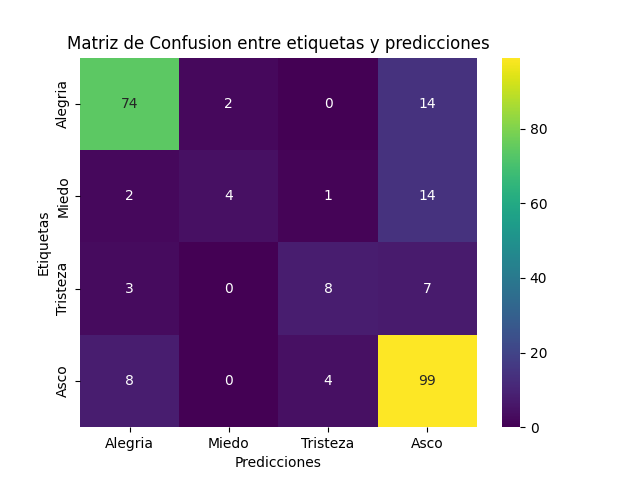
\includegraphics{Images & Logos/Results/Matriz_confusion.png} 
	\caption{Matriz de confusión entre etiquetas asignadas y predicciones del algoritmo para el dataset etiquetado}
	\label{figure:Matriz}
\end{figure}

Este fue el caso también para tristeza, como se aprecia en el tweet numero 2 de la tabla \ref{table:ejemplos_2}. Para Alegría se observa que también algunos fueron predichos como asco. Lo que ocurrió en muchos casos es que en un mismo tweet, se expresaban dos emociones distintas, una en cada frase, como se aprecia en el tweet numero 3 de la tabla.

\begin{table}
\caption{Ejemplos de tweets clasificados}
\label{table:ejemplos_2}
\begin{tabular}{{ | p{2cm} | p{13cm} |}}
\toprule
Numero de Ejemplo & Tweet \\
\midrule
1 & \#AColombiaLePreocupa es la relación de @AndresPastrana\_ con la Unión Temporal Disproel, que es la que hace el conteo corrupto desde hace más de 20 años. ¿Pasos de animal grande sobre el control de las elecciones? \\
2 & \#TodoVale por eso es que estamos anclados al subdesarrollo, por anteponer todo por los principios. Un mentiroso y sucio Petro no le importa hacer lo que sea con tal de ganar. Los fines no justifican los medios. Petro acabó la posibilidad de un proyecto alternativo por su ego \\
3 & Juan Roberto Vargas es una persona decente. Néstor Morales es una porquería de persona. \#DebateFinal \\
\bottomrule
\end{tabular}
\end{table}






\section{Distribución de emociones por sector}

Una vez desplegado el modelo y obtenido las etiquetas emocionales para todos los tweets del dataset, se obtienen los resultados obtenidos en el gráfico \ref{figure:tweets_total}, en donde se aprecia el porcentaje de tweets que recibió cada una de las distintas etiquetas. Allí puede apreciarse que la emoción mas preponderante fue el asco, con mas del 50\% de los tweets. Luego fue la alegría, con alrededor del  40\%. Finalmente, el miedo y la tristeza estuvieron mucho menos presentes con menos del 3\% cada una. 



\begin{figure}[t]
	\centering
	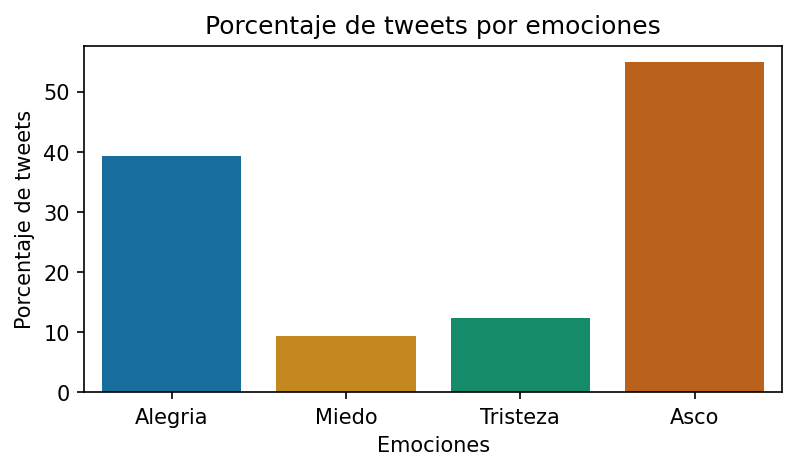
\includegraphics{Images & Logos/Results/Cantidad_de_tweets__por_emocion.png} 
	\caption{Porcentaje de tweets clasificado según emociones por el algoritmo}
	\label{figure:tweets_total}
\end{figure}



Al analizar la presencia de cada emoción en los distintos sectores políticos, se obtuvieron los resultados que se presentan en el gráfico \ref{figure:porcentaje_emocion}. En dicho gráfico se observa que el sector neutral fue el que mostró una mayor cantidad de tweets etiquetados con miedo, representando aproximadamente el 3\% de sus tweets. En cambio, tanto la izquierda como la derecha tuvieron una presencia menor, con alrededor del 1.2\% y 0.8\% respectivamente. En relación a  alegría,se revela que la izquierda fue el sector que mostró una mayor presencia de dicha emoción en sus tweets, alcanzando el 55\%. En segundo lugar se encuentra el sector neutral, con un 33\%, seguido por la derecha con un 29\%. En cuanto al asco, se destaca la participación predominante de la derecha, representando un 69\% del total de sus tweets. El sector neutral se posiciona en segundo lugar con un 54\% de los tweets, dejando a la izquierda con el menor porcentaje de los tres, un 40\%. Finalmente, para la tristeza, el sector neutro fue en donde esta emoción tuvo mayor presencia con un 5\% de su total, lo cual fue bastante mayor que la izquierda y la derecha, con un un .08 y .04\% respectivamente.



\begin{figure}[t]
	\centering
	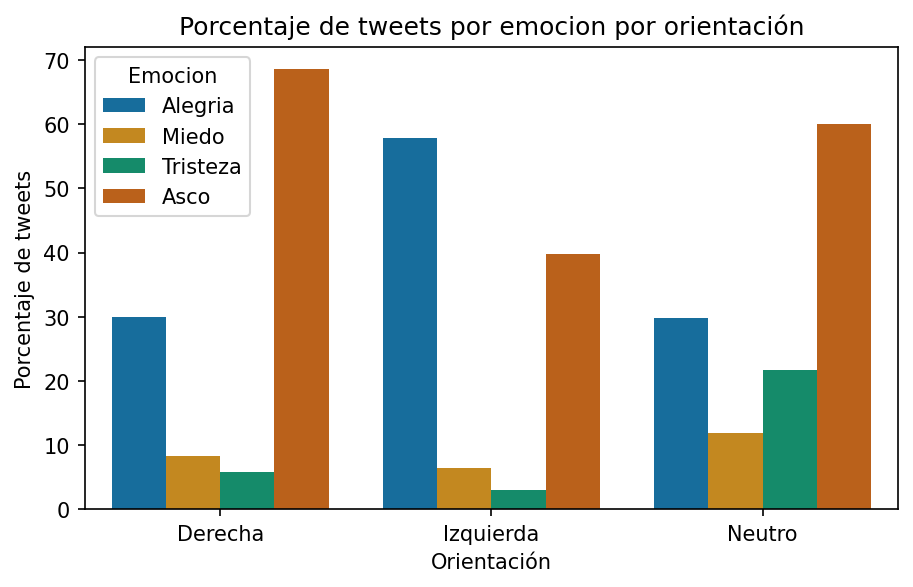
\includegraphics{Images & Logos/Results/Porcentaje de tweets por emocion por sector.png}
	\caption{Porcentaje de tweets clasificados según emoción por el algoritmo, separado por sector político del hashtag}
	\label{figure:porcentaje_emocion}
\end{figure}





\section{Emociones a lo largo del tiempo}


Para determinar en cada emoción, que porcentaje de esta etiqueta tuvo un día en particular, se  dividió el numero tweets con esta etiqueta en dicho día sobre el total de tweets con esta etiqueta. De esta manera, se aprecia en el gráfico  \ref{figure:tweets_percent_tiempo}, que el 29 de mayo fue particularmente activo pues contó con casi 40\% de los tweets con miedo, y un 26\% de los tweets con alegría y tristeza. Este fue el día de la primera vuelta presidencial. Del mismo modo, se aprecia como los días 9 y 10 de junio tuvieron un repunte de asco y tristeza respectivamente, con un 9 y 11\%. Estos días estuvieron marcados con el evento de los llamados Petro videos. Luego hay un repunte de asco y tristeza al rededor del 16 de junio, fecha en donde se hablo del debate final al cual Rodolfo Hernandez se negó a participar, y finalmente de alegría, tristeza y miedo para el 19 de junio que fue la segunda vuelta.

\begin{figure}[t]
	\centering
	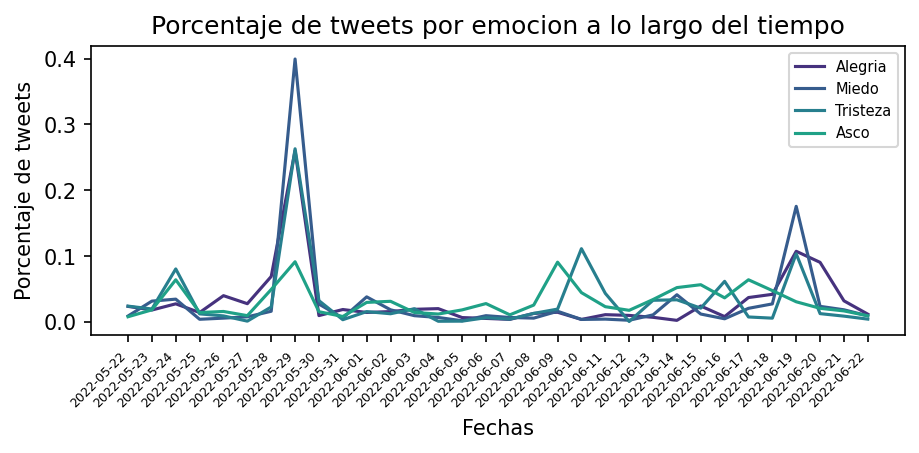
\includegraphics{Images & Logos/Results/Porcentaje de tweets por emocion a lo largo del tiempo.png} 
	\caption{Porcentaje diario del total de tweets clasificados en cada emoción a lo largo del tiempo}
	\label{figure:tweets_percent_tiempo}
\end{figure}



Para cada emoción y sector, se obtuvo que porcentaje de esta etiqueta tuvo cada sector un día en particular, al dividir el numero de tweets que este sector tuvo con cada etiqueta en dicho día sobre el total de tweets que este sector tuvo con esta etiqueta. De esta manera, se obtiene el gráfico \ref{figure:tweets_percent_alegria_tiempo} para alegría en donde se aprecia que el 29 de mayo todos los sectores tuvieron un repunte. Luego los tres sectores van creciendo cercanos al 19 de junio, para decaer eventualmente primero la derecha, luego el sector neutro y finalmente la izquierda.




\begin{figure}[t]
	\centering
	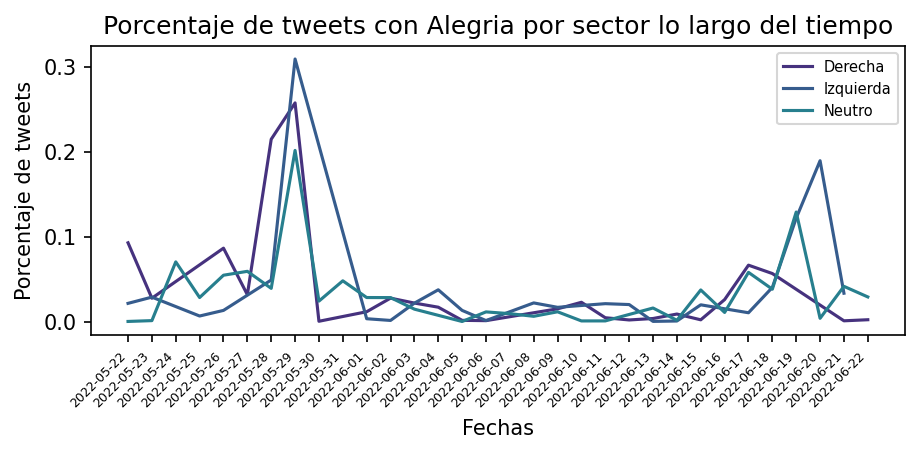
\includegraphics{Images & Logos/Results/Porcentaje de tweets con Alegria por sector lo largo del tiempo.png} 
	\caption{Porcentaje diario del total de tweets clasificados como Alegría, para cada sector político}
	\label{figure:tweets_percent_alegria_tiempo}
\end{figure}


Para el caso del miedo, se observa un gran pico de los tres sectores el 29 de mayo, día de la primera vuelta. Luego, para el 14 de junio, hubo un pico de miedo en la derecha como consecuencia a los rumores de estallido social, para finalmente haber un pico de miedo del sector neutro y de la izquierda cercano al 19 de junio.

\begin{figure}[t]
	\centering
	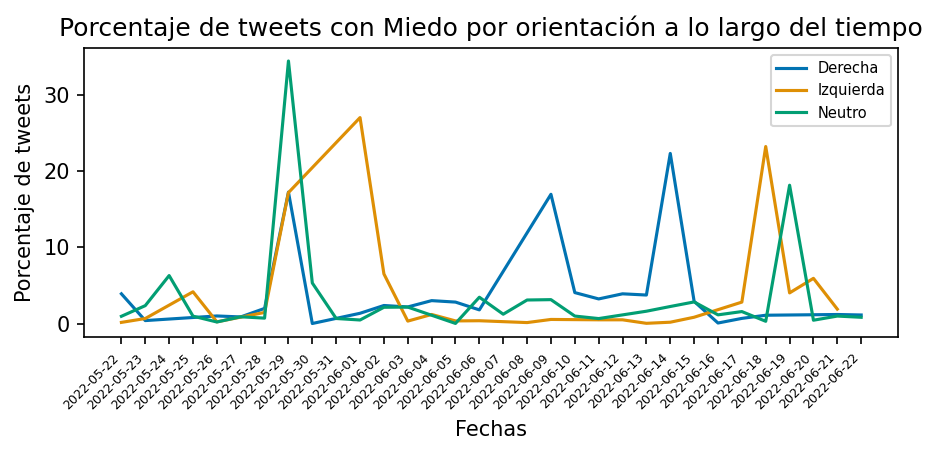
\includegraphics{Images & Logos/Results/Porcentaje de tweets con Miedo por sector lo largo del tiempo.png} 
	\caption{Porcentaje diario del total de tweets clasificados como Miedo, para cada sector político}
	\label{figure:tweets_percent_Miedo_tiempo}
\end{figure}


En cuanto a la tristeza, se aprecia que los tres sectores tuvieron un repunte el 29 de mayo, principalmente la izquierda en donde este día se llego a casi un 40\%. Luego el 9 de junio hubo un repunte en la derecha, ligado al evento de los petro videos, y luego el 10 un repunte del sector neutro en donde se discutieron temáticas decepcionantes de las elecciones. Para el 14 de junio, la derecha tuvo devuelta un repunte de tristeza ligado, al igual que para el miedo, a la temática del estallido social. Finalmente, los tres sectores tuvieron un incremento de la tristeza para el 19 de junio.

\begin{figure}[t]
	\centering
	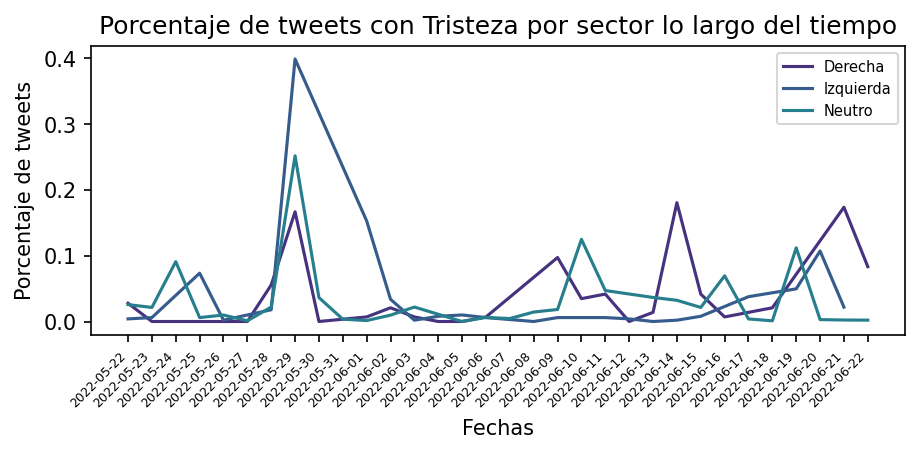
\includegraphics{Images & Logos/Results/Porcentaje de tweets con Tristeza por sector lo largo del tiempo.png} 
	\caption{Porcentaje diario del total de tweets clasificados como Tristeza, para cada sector político}
	\label{figure:tweets_percent_Tristeza_tiempo}
\end{figure}

En cuanto al asco, al inicio hay un pico del sector neutro el 24 de mayo debido a las reacciones respecto a un debate. Luego, hubo un repunte de los tres sectores para el 29 de mayo. Se destaca luego el gran pico que tuvo la derecha para el 9 de junio, fecha de los petro videos, con mas del 25\%. Asi mismo, se observa que la izquierda tuvo su pico el 17 de junio con cerca del 20\%. En esta fecha fue en donde se hablo de la negativa de Rodolfo Hernandez a participar en el debate final

\begin{figure}[t]
	\centering
	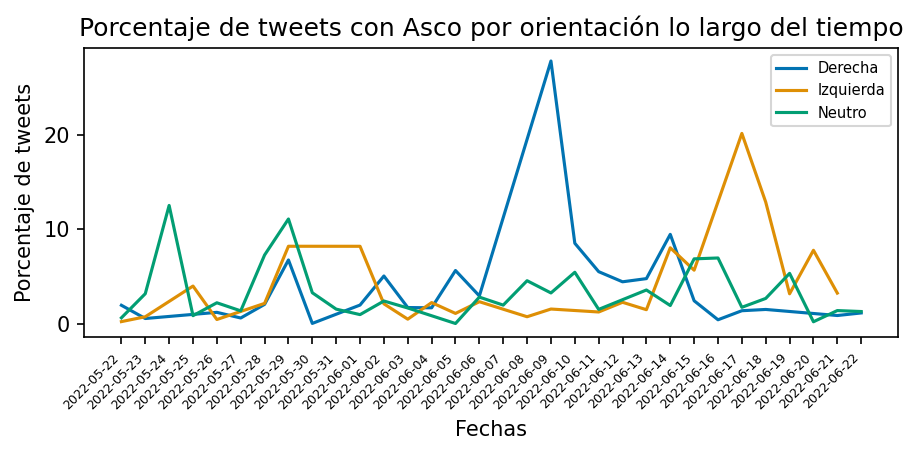
\includegraphics{Images & Logos/Results/Porcentaje de tweets con Asco por sector lo largo del tiempo.png} 
	\caption{Porcentaje diario del total de tweets clasificados como Asco, para cada sector político}
	\label{figure:tweets_percent_Asco_tiempo}
\end{figure}














